% THIS IS SIGPROC-SP.TEX - VERSION 3.1
% WORKS WITH V3.2SP OF ACM_PROC_ARTICLE-SP.CLS
% APRIL 2009
%
% It is an example file showing how to use the 'acm_proc_article-sp.cls' V3.2SP
% LaTeX2e document class file for Conference Proceedings submissions.
% ----------------------------------------------------------------------------------------------------------------
% This .tex file (and associated .cls V3.2SP) *DOES NOT* produce:
%       1) The Permission Statement
%       2) The Conference (location) Info information
%       3) The Copyright Line with ACM data
%       4) Page numbering
% ---------------------------------------------------------------------------------------------------------------
% It is an example which *does* use the .bib file (from which the .bbl file
% is produced).
% REMEMBER HOWEVER: After having produced the .bbl file,
% and prior to final submission,
% you need to 'insert'  your .bbl file into your source .tex file so as to provide
% ONE 'self-contained' source file.
%
% Questions regarding SIGS should be sent to
% Adrienne Griscti ---> griscti@acm.org
%
% Questions/suggestions regarding the guidelines, .tex and .cls files, etc. to
% Gerald Murray ---> murray@hq.acm.org
%
% For tracking purposes - this is V3.1SP - APRIL 2009

%\documentclass{acm_proc_article-sp}
\documentclass{sig-alternate}
\usepackage[numbers, sort, compress]{natbib}
\usepackage{graphics}
\usepackage{graphicx}
\usepackage{epstopdf}
\usepackage{color}
\usepackage{hyperref}
\usepackage{pdfsync}
\usepackage{mdwlist}

\begin{document}

\conferenceinfo{TeraGrid 11} {}
\CopyrightYear{2011}
\crdata{}
\clubpenalty=10000
\widowpenalty = 10000


%\title{A Sample {\ttlit ACM} SIG Proceedings Paper in LaTeX
%Format\titlenote{(Does NOT produce the permission block, copyright information nor page numbering). For use with ACM\_PROC\_ARTICLE-SP.CLS. Supported by ACM.}}

\newif\ifdraft
\drafttrue                                                                                                   

\ifdraft
% \newcommand{\reviewer}[1]{ {\textcolor{blue}    { ***Reviewer:     #1 }}}
 \newcommand{\jkimnote}[1]{{\textcolor{green}   { ***Joohyun:   #1 }}}
 \newcommand{\jhanote}[1]{  {\textcolor{red}     { ***SJ: #1 }}}
  \newcommand{\smnote}[1]{  {\textcolor{red}     { ***Sharath: #1 }}}
 \newcommand{\todo}[1]{  {\textcolor{red}     { ***TODO: #1 }}}
 \newcommand{\fix}[1]{  {\textcolor{red}     { ***FIX: #1 }}}
 \newcommand{\reviewer}[1]{}
\else
 \newcommand{\reviewer}[1]{}
 \newcommand{\jkimnote}[1]{}
 \newcommand{\smnote}[1]{}
 \newcommand{\jhanote}[1]{}
 \newcommand{\todo}[1]{  {\textcolor{red}     { ***TODO: #1 }}}
 \newcommand{\fix}[1]{}                                                                                     
\fi

\title{Building Gateways for Life-Science Applications using the
  Distributed Adaptive Runtime Environment (DARE) Framework}

%\subtitle{[Extended Abstract]
%\titlenote{A full version of this paper is available as
%\textit{Author's Guide to Preparing ACM SIG Proceedings Using
%\LaTeX$2_\epsilon$\ and BibTeX} at
%\texttt{www.acm.org/eaddress.htm}}}
%
% You need the command \numberofauthors to handle the 'placement
% and alignment' of the authors beneath the title.
%
% For aesthetic reasons, we recommend 'three authors at a time'
% i.e. three 'name/affiliation blocks' be placed beneath the title.
%
% NOTE: You are NOT restricted in how many 'rows' of
% "name/affiliations" may appear. We just ask that you restrict
% the number of 'columns' to three.
%
% Because of the available 'opening page real-estate'
% we ask you to refrain from putting more than six authors
% (two rows with three columns) beneath the article title.
% More than six makes the first-page appear very cluttered indeed.
%
% Use the \alignauthor commands to handle the names
% and affiliations for an 'aesthetic maximum' of six authors.
% Add names, affiliations, addresses for
% the seventh etc. author(s) as the argument for the
% \additionalauthors command.
% These 'additional authors' will be output/set for you
% without further effort on your part as the last section in
% the body of your article BEFORE References or any Appendices.

\numberofauthors{6} %  in this sample file, there are a *total*
% of EIGHT authors. SIX appear on the 'first-page' (for formatting
% reasons) and the remaining two appear in the \additionalauthors section.
%
\author{
% You can go ahead and credit any number of authors here,
% e.g. one 'row of three' or two rows (consisting of one row of three
% and a second row of one, two or three).
%
% The command \alignauthor (no curly braces needed) should
% precede each author name, affiliation/snail-mail address and
% e-mail address. Additionally, tag each line of
% affiliation/address with \affaddr, and tag the
% e-mail address with \email.
%
\alignauthor Joohyun Kim\\
       \affaddr{Center for Computation and Technology}\\
       \affaddr{Louisiana State University}\\
       \affaddr{216 Johnston}\\
       \affaddr{Baton Rouge, LA} \\
       \email{jhkim@cct.lsu.edu}
\alignauthor Sharath Maddineni\\
       \affaddr{Center for Computation and Technology}\\
       \affaddr{Louisiana State University}\\
       \affaddr{216 Johnston}\\
       \affaddr{Baton Rouge, LA}
       \email{smaddineni@cct.lsu.edu}
\alignauthor Shantenu Jha\titlenote{Author for correspondence}\\
      \affaddr{Center for Computation and Technology}\\
     \affaddr{Louisiana State University}\\
      \affaddr{214 Johnston}\\
      \affaddr{Baton Rouge, LA}
     \email{sjha@cct.lsu.edu}
}
% There's nothing stopping you putting the seventh, eighth, etc.
% author on the opening page (as the 'third row') but we ask,
% for aesthetic reasons that you place these 'additional authors'
% in the \additional authors block, viz.
%\additionalauthors{Additional authors: John Smith (The Th{\o}rv{\"a}ld Group,
%email: {\texttt{jsmith@affiliation.org}}) and Julius P.~Kumquat
%(The Kumquat Consortium, email: {\texttt{jpkumquat@consortium.net}}).}
\date{22 April 2011}
% Just remember to make sure that the TOTAL number of authors
% is the number that will appear on the first page PLUS the
% number that will appear in the \additionalauthors section.

\maketitle


\begin{abstract}
  We introduce the Distributed Adaptive Runtime Environment (DARE)
  framework that is a SAGA-based higher-level abstraction, and
  demonstrate its effectiveness as an integral component of a
  wide-range of life-science Gateways.  An understanding of challenges
  and computational requirements of the life science applications in
  distributed heterogeneous scalable HPC resources has led to the
  development of the DARE framework with which a lightweight,
  extensible, versatile Gateway that seamlessly utilizes scalable
  infrastructure can be built for a life science application
  effectively.  DARE science gateways comprise a user access layer,
  built upon Simple API for Grid Application (SAGA) and the SAGA-based
  Pilot-Job (SAGA-BigJob) capability.  This work is predicated on
  three important trends: (i) the importance, impact and percentage of
  TeraGrid/XD resources assigned to the life-sciences is increasing at
  a rate that is probably greater than other disciplines, (ii) that
  Gateways have proven to be a very effective access mechanism to
  distributed HPC resources provided by the TG/XD, and in particular a
  very successfull model for shared/community access models, and (iii)
  that there are missing capabilties and abstractions to enable the
  use of the collective capacity of distributed cyberinfrastructure
  such as TG/XD, especially those that can be used to develop Gateways
  in an easy, extensible and scalable fashion for both
  compute-intensive and data-intensive applications.  We present the
  framework and four specific life science gateways -- DARE-RFOLD,
  DARE-DOCK, DARE-HTHP and DARE-NGS, that allow a user to carry out
  RNA secondary structure prediction, virtual screening using a
  docking method, large-scale ensemble-based molecular dynamics
  simulations and alignment of Next-Genartion DNA sequencing data on a
  reference genome respectively.

  % We use DARE as the underlying component for four different
  % Gateways that use both TG/XD resources as well as LONI
  % The middleware, in particular, owing to the core features provided
  % by SAGA such as interoperability, distributed scale-out,
  % extensibility, adaptivity, and simplicity (IDEAS) and a pilot job
  % abstraction, SAGA-BigJob,; facilitates a gateway developer to
  % implement a various execution patterns as well as distributed data
  % management.  By employing the DARE framework as well as the
  % SAGA/SAGA-BigJob, science gateways is able to provide a target
  % scientific application whose capacity is immediately enhanced with
  % distributed scalable HPC resources such as Teragrid and other
  % emerging computing environments such as clouds, consequently
  % advancing scientific computing, for example, by providing suitable
  % solutions for challenges in data-intensive scalable computing.

\end{abstract}

\category{D.1.3}{Software}{Concurrent Programming}{ Distributed programming/parallel programming} 
\category{J.3}{Computer Applications}{Bioinformatics}


% A category with the (minimum) three required fields
%\category{H.4}{Information Systems Applications}{Miscellaneous} %Acategory including the fourth, optional field follows...
%\category{D.2.8}{Software Engineering}{Metrics}[complexity measures,performance measures]

\section*{General Terms}{Design,Measurement,Theory}

 \keywords{Science Gateway, Runtime Environment, Distributed Computing, Simple API for Grid
  Applications (SAGA), Pilot-Job abstraction}

%\keywords{ACM proceedings, \LaTeX, text tagging} % NOT required for Proceedings 
%\keywords{RNA conformation energy landscape, Runtime Environment, SAM-I riboswitch,
% S gene of Bovine Corona Viral Genome} % NOT required for Proceedings




\section{INTRODUCTION}

\subsection{TeraGrid Usage by the life science community}

The importance of computing in the life-sciences has been well
documented. An interesting corollary is that the rate-of-increase of
computing resources devoted to the life-sciences is increasing, and
increasing at a rate faster than any other discipline. 

It is difficult to provide such information in a consistent way
as the total number of cycles avaialable year-to-year varies, but
also which discipline a proposal gets assigned to is somewhat
random; thus many chemistry proposals, even physics proposals
are likely to be biological in nature. 

In spite of fundamental limitations on the accuracy of the data,
as seen from Fig~\ref{tg2007, tg2008} the trends are somewhat
unabmigious: the percentage of TeraGrid resources devoted
to the life-sciences is already more than any discipline and
the usage seems to be increasing on the back of other disciplines, 
whether measured by number of cycles consumed, users or 
allocations.

% The single largest community is the life-sciences community --
% including MD (25\%)...  Get a break-down of the total usage of the TG
% by discipline and application type.


\begin{figure}
 \centering
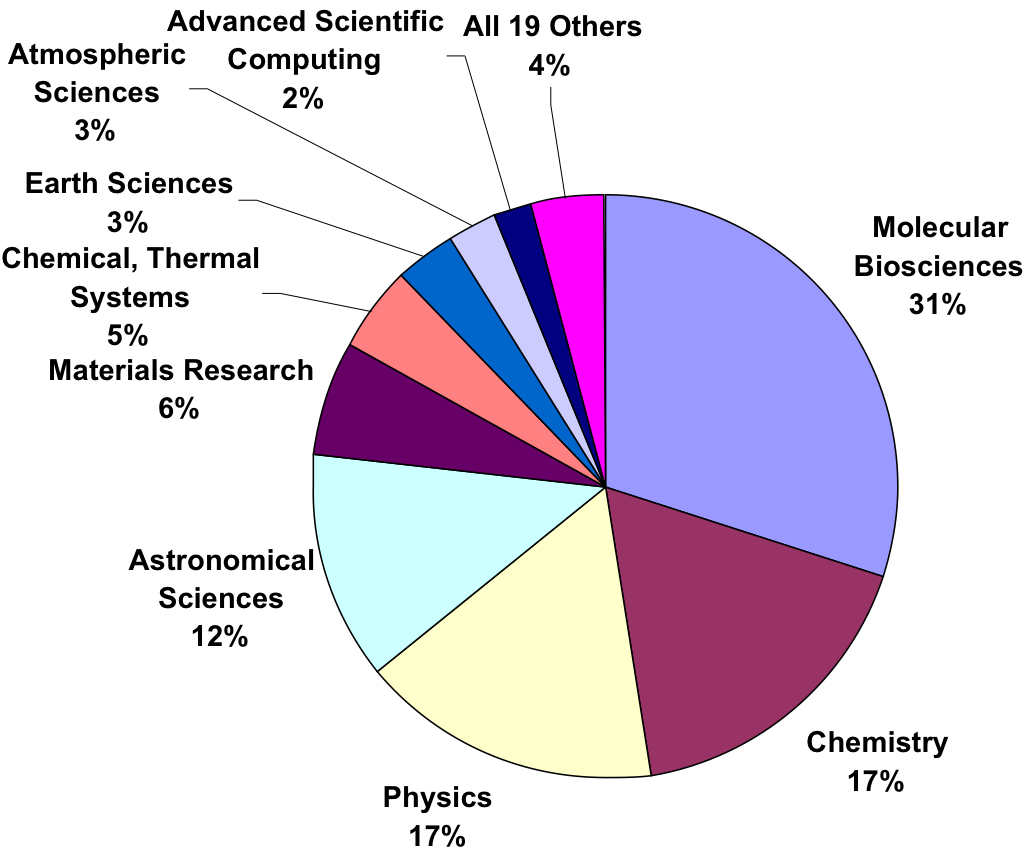
\includegraphics[scale=0.40]{figures/teragrid-discipline07}
\caption{\small 2007 Usage statistics for the TeraGrid} 
  \label{tg2007}
\end{figure}


\begin{figure}
 \centering
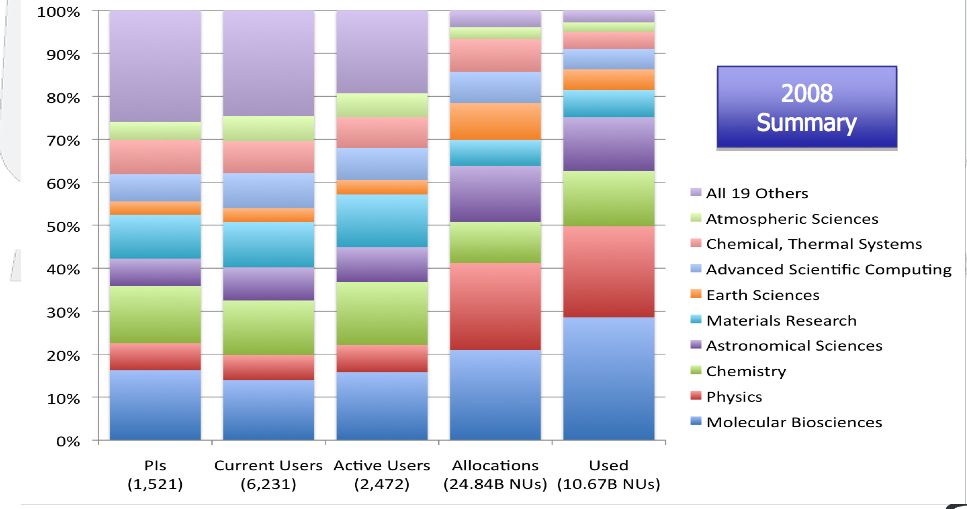
\includegraphics[scale=0.27]{figures/teragrid-discipline08}
\caption{\small 2008 Usage statistics for the TeraGrid}
  \label{tg2008}
\end{figure}


\subsection{Large scale life science applications on the distributed HPC resources}
Traditionally, life science applications have been regarded as non-HPC
applications.  Only a few applications were actively pursued with
large scale computations.  Two representative examples are molecular
simulations and virtual docking calculations.  Interestingly, while
the former represents the case that the so-called scale up of bulk
synchronous techniques such as MPI is used as a main strategy for
large molecular systems, the latter represents the case that massive
independent tasks should be carried out, implying two different
application usage modes.

Meanwhile, the need of large-scale distributed parallel executions for
other life science applications has grown due to the advances of
experimental techniques using high-throughput approaches as well as
the advent of computing power and data management capacity.  For
example, Next-Generation DNA Sequencing (hereafter, NGS) technologies
challenge computational biology with unprecedented amounts of data
produced by their high-throughput capability.  Required data analytics
for processing such sequenced data along with dealing with genome data
sets available in public and private databases is overwhelmed by the
pace of growing data volume.  This poses the question on how the
challenge of large volume data-management as well as the requirement
of analyzing large volumes of data are effectively handled.

Interestingly, the cyberinfrastructure considerations requried to
support a broad-range of analytical approaches and at the scales
required, has received less attention that the data-management problem
and algorithmic advances.  Thus not surprisingly, traditional
production cyberinfrastructure, such as the TeraGrid, have not been
used for such data-intensive analytics. There are multiple reasons,
but a couple of contributing factors are: (i) insufficient runtime
enviroments (and abstractions) to support concurrent computational
capabilties with large-data sets to support data-analytics (beyond
visualization) in an easy, scalable and extensible fashion, (ii)
insufficient support for user-customizable data-intensive "workflows"
that effectively hide the challenges of data-movement and efficient
data-management whilst managing concurrent distributed (computational)
resources.

Indeed, molecular simulations, virtual screening, and many other bioinformatics applications, particularly, regarded as the non-HPC applications could increase their usages dramatically by utilizing distributed scalable resources, which is, as presented in this work, addressed by a gateway development that implements a runtime environment for executions of target computation and distributed data management.


This work is predicated on three important trends: (i) the importance,
impact and percentage of TeraGrid/XD resources assigned to the
life-sciences is increasing at a rate that is probably greater than
other disciplines, (ii) that Gateways have proven to be a very
effective access mechanism to distributed HPC resources provided by
the TG/XD, and in particular a very successfull model for
shared/community access models, and (iii) that there are missing
capabilties and abstractions to enable the use of the collective
capacity of distributed cyberinfrastructure such as TG/XD, especially
those that can be used to develop Gateways in an easy, extensible and
scalable fashion for both compute-intensive and data-intensive
applications. We introduce the DARE framework that is a SAGA-based
higher-level abstraction, and demonstrate its effectiveness as an
integral component of a wide-range of life-science Gateways. We
use DARE as the underlying component for four different
Gateways that use both TG/XD resources as well as LONI resources.






\subsection{Challenges in developing a gateway supporting distributed applications with heterogeneous multiple HPC resources}

Science gateways, in particular, utilized for the Teragrid community, have witnessed their successful achievements with the growth of the number of supporting researchers and computing time usages.  However, most of gateways are not likely to consider a distributed application as a primary target.  Perhaps, a big reason is due to additional complexity with a distributed application.  Nonetheless, the main developmental objectives for distributed applications are generally to achieve the key features such as interoperability, distributed scale-out, extensibility, adaptivity, simplicity-taken together referred as IDEAS.  Achieving such goals are, however, not trivial mainly due to the lack of tools for the coordination over multiple and distributed compute/data sites.  As we observe with the advent of federated grids such as Teragrid and its transition to eXtreme Digital (XS) environment, such requirements become harder to achieve as the number of connected sites grows as well as the computing power and the data storage capacity of each resource reach peta or exa scales.   More importantly, supporting a broad range of diverse execution patterns is critical considering different application usage modes for different life science applications.  For example, in Table~\ref{table:four-applications}, application usages for four life science applications focused on this work are summarized by contrasting conventional vs. distributed modes.  Last not the least, it is always challenging to respond effectively for upcoming demands of supporting new applications, distributed data management with new infrastructure, implementation of novel execution patterns, which is often eased by the development of a framework and its use for the efficiency in development cycle.   



\section{FOUR LIFE SCIENCE APPLICATIONS}

\begin{table}
\small
\begin{tabular}{|c|c|c|c|} 
  \hline Science  & Supported  & Conventional   & Example of  
  \\
  Domain & Appli- & Application & Distributed Application \\ 
  &  cation(s) & Usage Mode & Usage Mode \\  \hline \hline 
  
  Molecular   &  \texttt{NAMD} &  MPI-based  & ensemble-based   \\
   Dynamics  &  & single cluster execution & multiple (independent/ \\ 
   &  &  &  loosely-coupled)  \\ 
   &  &  &  execution \\ \hline
  RNA   & \texttt{SFOLD}, & single node   & multiple tasks with \\
  Folding   & \texttt{RNAFold} & serial execution &   distributed resources \\
  Prediction & &  & \\ \hline
  NGS data     &  \texttt{BFAST} & memory-intensive  & data-intensive\\ 
     analytics  &  &  single node execution   &  distributed resources \\ \hline
  Virtual  & \texttt{Autodock} &  many tasks   & many tasks \\
   Screening  &  & with a cluster  & with multiple resources \\
  (Docking) &  &  & \\ \hline

\hline
\end{tabular} \caption{Four life science applications and their usage modes.  Four gateways for the applications were developed with the DARE framework}
 \label{table:four-applications} 
\end{table}

% \bibliographystyle{plain}
% \bibliography{egi-white-paper}

%\begin{figure}
% \centering
%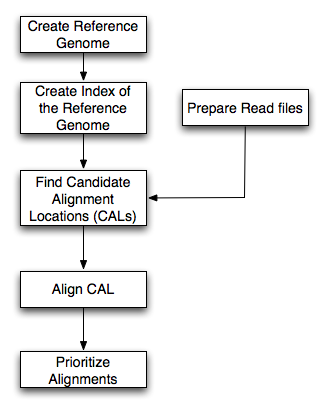
\includegraphics[scale=0.45]{figures/workflow.png} 
%
%\caption{\small Overall workflow for a mapping procedure using BFAST.  In this work, we focus on the step for finding Candidate Alignment Locations (CALs).  }
%  \label{fig:workflow-bfast} 
% \end{figure}
%
%
%\begin{table}
%\begin{tabular}{|c|c|c|c|} 
%  \hline 
% BFAST command & Description & Features for \\ 
%  &  &     Parallelism \\ \hline \hline
%\texttt{bfast fasta2brg} & creation of a ref. genome  &    multiple independent contigs \\ \hline 
%\texttt{solid2fastq}  &  preparation of short reads files &     multiple sequence reads files \\ \hline
%
%\texttt{bfast index} & creation of reference genome indexes& multi-threading and  \\
% &   & low memory option  \\  \hline
%\texttt{bfast match} & finding candidate alignment locations  &  multi-threading and  \\
%& &  parallel execution \\ \hline
%\texttt{bfast localalign} & alignment of each CAL  &   parallel execution \\  \hline
%\texttt{bfast postprocess} & prioritization of alignments  &  parallel execution \\ \hline
%
%
%\hline
%\end{tabular} \caption{Description of BFAST commands and features for parallel and multi-threading execution}
% \label{table:bfast-summary} 
%\end{table}
%


Here we introduce the four scientific applications briefly describing the focus features provided by the gateways

\textit{Large scale Molecular Dynamics simulations}

Over the past two decades, the field of biomolecular simulation has
exploded due to increases in computational power and parallel codes,
the emergence of accurate molecular mechanical potentials or force
fields and improvements in the methods~\cite{cheatham-1,
  cheatham-2}. A continually growing body of researchers apply
atomistic and coarse-grained molecular dynamics (MD) simulation
methods to facilitate drug discovery, perform advanced materials
research, to design and understand biomolecular and designed
catalysts, and to provide fundamental insight into molecular
structure, dynamics and interactions. 

%Particular challenges include de
%novo protein and nucleic acid folding and structure prediction;
%correctly modeling induced-fit and conformational selection as drugs
%or other molecules interact with a target macromolecule; modeling
%large ensembles of biomolecules such as proteins in a membrane
%environment, viruses, and biomolecular machines such as the ribosome;
%combined quantum and molecular mechanical treatments for modeling
%chemistry; and improving conformational sampling and estimation of
%free energies and free energy pathways. 

In response to the perceived needs and importance of molecular
simulations, numerous high performance distributed memory parallel codes
have emerged in the past two decades (including NAMD~\cite{cheatham-3},
CHARMM~\cite{cheatham-4}, AMBER~\cite{cheatham-5},
LAMMPS~\cite{lammps}GROMACS~\cite{cheatham-6}, etc.), and many now can
directly include quantum representations. 





\textit{NGS-driven genome data analytics}
In the past several years, there has been a major paradigm shift in biological/biomedical researches with the Next-Generation DNA Sequencing technologies\cite{mardis2008-tig,metzker2010,mardis2008-arghg}.  Their novel capabilities of cost-effective resequencing, full-scale quantitative transcriptomics, and holistic approach for cell development and cell differentiation using protocols such as RNA-seq. and ChIP-seq opens a completely new era for life science researches\cite{sorek2010,mortazavi2008}.  In spite of such great opportunities, current NGS platforms challenges data analytics to deal with the sequencing data and the following bioinformatics analysis and inference.  For example, at this moment, NGS platforms produce typically billions of reads that comprise a short sequence mostly less than 100 base pairs with most of real experimental setting\cite{alex2009,trapnell2009}.  Furthermore, the increasingly effective cost-down trend causes the difficulty in management of significant size of data produced or related data sets that should be analyzed together.  
Generally, bioinformatics tools or applications developed for NGS data analytics are numerous and there is no sign to see the end of influx of new tools considering continuous innovations in the technologies and algorithmic advances in such tools.  In particular, we focus on the  important analysis of NGS data, mapping of NGS data reads on a reference genome.  It is noted that this analysis step should be applied first to proceed the following analyses targets more specific research goals such as genome variation, genome-wide association, comparative genomics, and other applications for investigating biological processes in a living cell.     



\textit{RNA structure prediction and beyond}
Defying the old biological dogma, positioning RNAs as a genome information intermediate between DNAs and proteins, during the last couple of decades, the number of scientific observations found that RNAs were involved significantly in gene expression and regulation\cite{joyce1999,cruz2009,encode2007,amaral2008}.  Now, with the well-known categories of non-coding RNAs such as miRNAs and riboswitches, in spite of their biogenesis that does not need to be translated into proteins, significant roles of RNAs are quite well recognized\cite{costa2009,ellington2007,baek2008,blouin2009,henkin2009}.  Importantly, RNA functions by forming required structure(s), and the pattern of structure formation of RNAs are somewhat contrasted to proteins that are mostly folded into highly specific 3-D structure\cite{roth2009}. For example, riboswitches chose one of two alternative structures, in response to meta-bolite binding, consequently resulting in two different gene regulation stages, i.e., turning on downstream gene synthesis or turning it off\cite{montange2008,dambach2009,weinberg2007}.  Therefore, RNA structure prediction has been the major area for RNA studies and may noticeable progresses were made recently for RNA 2D structure prediction as well as 3D structure modeling\cite{shapiro2007,mathews2006,ding2003}.   




\textit{Drug Discovery via Virtual Screening strategies}
For small molecule drug discovery, virtual screening using a docking method has been widely utilized and an immediate requirement for massive docking calculations against a chemical database has been attempted by managing such many tasks using a local cluster, HPC cluster, grids, and clouds\cite{levesque2009,yim2010}.  The nature of required application usage mode for virtual screening methods is a generic example of many task computing, implying that pleasingly parallel massive tasks carrying out a docking computation should be executed.  In spite of such well-established protocol, the challenges in drug discovery finding putative inhibitors for target receptors are not resolved due to intrinsic difficulties with underlying physico-chemical models associated with the issues with scoring function, receptor flexibility, and docking strategy itself\cite{amaro2010}.  Therefore, more computing power and scaled calculations by varying the parameters for virtual screening are needed in order to understand the accuracy of results, suggesting the need of scalable infrastructure is highly appreciated while the application usage mode is generally intact.   





\subsection{Computational requirements and challenges}

A growing limitation in the applications of life sciences is that workflow, data management, and
analysis have become rate limiting steps: what is missing is support for the end-to-end execution requirement of applications.

We also need to move to tiered sets of computational resources.  For
example, one can imagine running large ensembles of MD engines on
tightly coupled parallel machines (like Ranger or Kraken) with
real-time data streamed to separately running analysis and
visualization resources (Lonestar, Spur), with on-the-fly monitoring
to analyze convergence, interesting phenomena or problems.  This also
provides the means for possible steering, for example by spawning or
stopping separate elements of the ensemble to sample more or less in a
particular region of interest.  In addition to real time monitoring,
hidden correlations in the data require the saving of coarser grained
simulation data on longer term (1-2 year) disk resources for further
analysis and mining using less tightly coupled computational
resources, and ultimately placing reduced and derived data sets
seamlessly back to the campuses, archivers, and for public
distribution.  Not only does this support the need for diverse sets of
computational resources, large-scale storage and data transfer
requirements for sophisticated analysis and visualization, and
high-bandwidth networking, it also drives the need for software tools
that facilitate the complicated workflow management, that allow
dynamic monitoring, starting and stopping of ensemble elements without
losing access to the global communications fabric and local
connections, and that provide the means for facilitating data
management and analysis.

In essence, the move from executing an individual task to \textit{large
  ensembles} of coupled/loosely/uncoupled tasks requires scientists to spend
significant time on compute and data management problems, instead of
core science.  The quantitative shift (massive distributed parallel
compute and data resources) implies qualitative change in the way how life science applications are being served for scientific discovery. 

\jhanote{At the end we propose DARE based Gateways as a solution}


\section{DISTRIBUTED ADAPTIVE RUNTIME ENVIRONMENT}
In order to provide a means for end users to utilize a scientific application with scalable heterogeneous distributed computing resources, we develop the Distributed Adaptive Runtime Environment (DARE) framework\cite{dareurl}.  As shown in Fig.~\ref{fig:dare-arch}, the framework comprises the access layer, the services layer, and the resource/provisioning layer.  Particularly, the core parts of the service layer and the resource/provisioning layer are powered by SAGA and SAGA pilot job abstraction, SAGA-BigJob\cite{saga-ccgrid10,saga-royalsoc,saga-web,jha2009developing,ecmls10, ecmls11}.  The access layer is built upon the open source web application framework, pylons\cite{pylonsurl}.  This combination of the open source technology and the application management system is the main design strategy behind the DARE framework for the development of a lightweight, extensible, full-fledged distributed computing science gateway quickly and effectively\cite{pylonsurl}. 

\subsection{SAGA and BigJob abstraction}
SAGA is an API providing the basic functionality for developing distributed applications, tools and frameworks\cite{saga-web}. The key advantages of the development using SAGA include i) to provide a general-purpose common functionality while hiding complexity of heterogeneity of back-end resources ii) to provide building blocks for constructing higher-level functionality and abstractions iii) to provide the means for developing broad range of distributed applications such as gateways, workflows, application management systems, and runtime environments.   Interestingly, SAGA provides a simple way to support python scripting for building distributed applications via python-binding.  SAGA-BigJob was introduced for a pilot-job abstraction with which various execution patterns and application usage modes are implemented.  Previously, we demonstrated the capabilities of SAGA-BigJob for scientific applications categorized as pleasingly parallel applications and loosely coupled applications\cite{saga-royalsoc,jha2009developing, ecmls10}

With the framework built upon SAGA and SAGA-BigJob, the fundamental design objectives of Interoperability across different infrastructure, Distributed Scale-Out, Extensibility, Adaptivity whilst preserving Simplicity (IDEAS), which constitutes essential requirement for distributed applications, are achieved in a remarkably effective way.


\subsection{Architecture : The Three Layers -- Access Layer, Services Layer and Resource /Provisioning Layer}
The architecture of DARE framework (see Fig.~\ref{fig:dare-arch}) assumes two-tier or three-tier installation scenarios that differ in the access layer such that the former does not need a remotely accessing client.  The access layer managed by web server using pylons and the application management system layers composed of the application layer, the dare layer, and SAGA layer reside on the server.  The middleware and resource layer represents the SAGA adaptors and back-end scalable distributed systems.  


\begin{figure}
 \centering
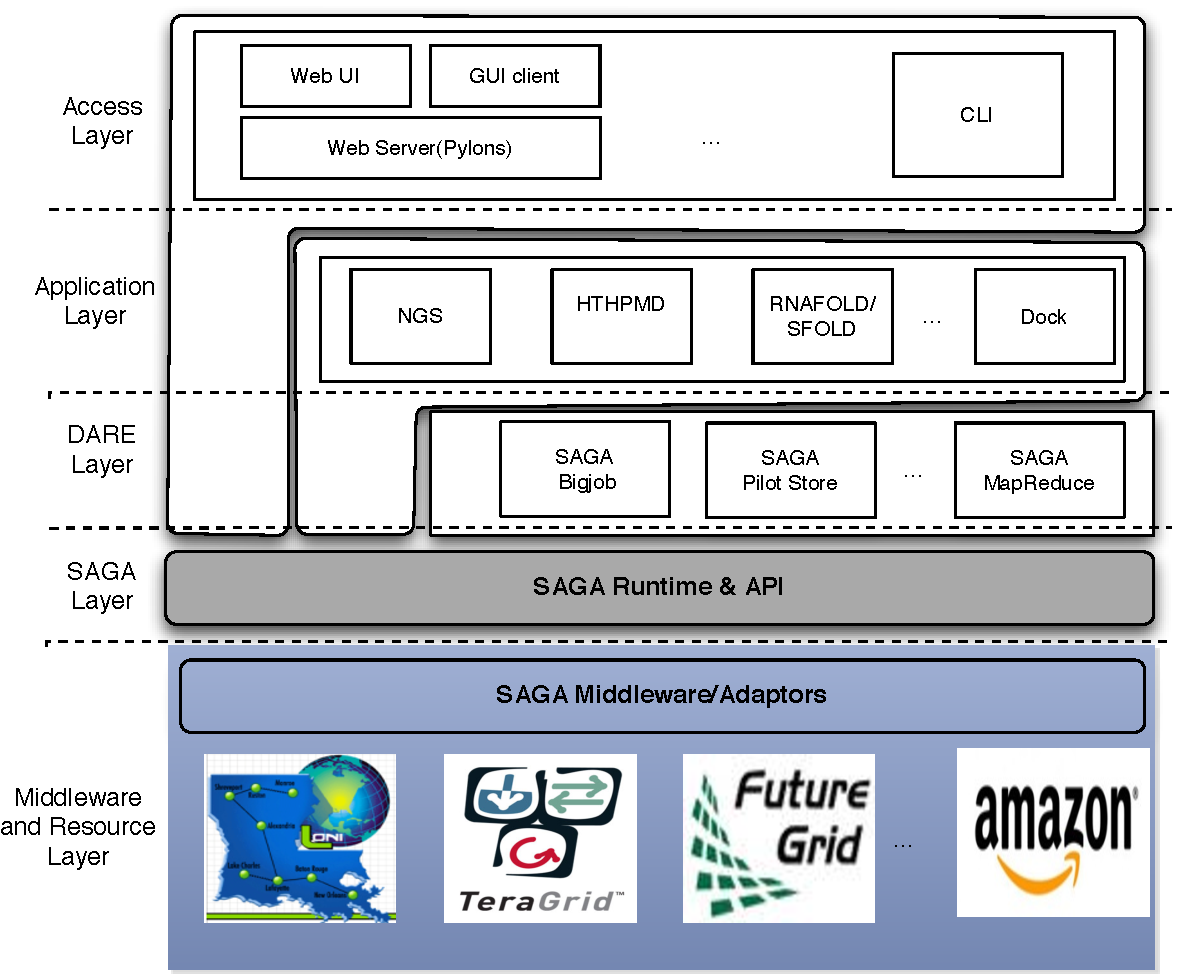
\includegraphics[scale=0.40]{figures/DAREOutline.pdf}

\caption{\small Dare architecture.}
  \label{fig:dare-arch} 
\end{figure}

 

%Level 2: (i) Computational aspect, (ii) Data management and movement, 
%
%Level 1: (iii)providing user interface


\textit{Access Layer} User interface for Web ,  Authentication, Job Management, Data Management, Remote or Distributed Job Submission these components are the heart of the DARE or any science gateway application further connecting these components to work in tandem is also an important issue.Lets start by understanding each component and worry about connecting them later.  Easily usable web interface for user is the main thing because thats what ultimately matters. So, for users with dare does not have to worry about how data is transferred , how job submissions should be used. So by using Pylons a MVC framework we design mako templates for users to submit their jobs and upload file there it self.

Authentication also plays an important role and prevents us from potential threads. So we utilize pylons authentications forms and provide user login and job management system.

\textit{Services Layer}

We have all this new jobs submitted from different users how are we going to decide where these jobs need to be run. There is also need for local job scheduler to intelligently decide for jobs that are submitted from the users. Sometimes jobs might be very short runs in this case we run them directly on the server locally.

Further, users may upload files from the web interface then first we need to save them locally and move them to multiple resources depending on the configuration and once the jobs are done we need to provide the users to help download them onto their machine for analyzing.

The meat of this framework is to be able run the jobs remotely this is addressed by utilizing the SAGA BigJob framework which provides an API to run the user submitted jobs remotely.


The web interface will be connected to remote job submission via a job scheduling and monitoring thread. This thread starts with pylons application and continuously communicates with local database server to find new jobs and it also acts as a scheduler for new jobs. Once this thread finds a new jobs it will start preparing the configuration files for that particular job from the user and afterwords it will start the remote job submission via application specific SAGA-Bigjob.

The data movement is also integrated into the application specific Bigjob because the movement of number of files, type of file will be changing from application.


All the above components are well connected but loosely coupled from each others as well so this provides the development of different kinds applications very simple and fast.

\textit{Resource/Provision Layer}


\section{FOUR DARE-BASED GATEWAYS}
\subsection{DARE-NGS}
Our DARE-NGS gateway (http://cyder.cct.lsu.edu/dare-ngs) supports Genome-wide analysis on Teragrid and provides currently the mapping process using BFAST that aligns the large number of short reads sequenced from NGS machines onto a reference genome sequence, which is the first step in scientific discovery utilizing NGS sequencing-based protocols such as the whole genome resequencing, RNA-seq, and ChIP-seq.  De novo assembly without reference genome information is still in early stages.  Note that due to its design strategy, including other analysis tool such as assembly or extending to a pipeline with other tools successively applied after the mapping with DARE-NGS are straightforward and underway at this moment.

It is worth mentioning that the computational complexity
of the analysis (e.g. mapping) depends, upon other things, the size
and complexity of the reference genome and the data-size of short reads.
Given that these can vary significantly, the computational
requirements of NGS-analytics also varies (even between data-sets of
similar size).  Thus an efficient, scalable and extensible analytical
approaches must be supported by any framework supporting
NGS-analytics.  The current service provided by DARE-NGS focuses mainly on the mapping step among bioinformatics tools with BFAST for single end NGS data or BFAST+BWA for paired-end data, and eventually supports a pipeline including genome variation studies for finding SNPs and small Indels.

Recently, we reported our exploration of NGS analytics using DARE-NGS with the HPC grid such as TeraGrid and
Cloud environment of FutureGrid\cite{ecmls11}.   

 \begin{table}
 \small
 \begin{tabular}{|c|c|c|c|c|c|c|} 
 \hline 
  Genome &Total             & $T_C$ (S)          & $T_C$  (S)  & $T_{C}$(S) &  $T_C$(S) & $T_{C}$ (S)  \\
  Type          &Cores           &  (R1)                     & (R2)              &  (R1,R2)       &  (R3)        & (R1,          \\
 &  &  &  &  &  &  R2,R3) \\ \hline
 B. Glumae   &   32 &          719               &      1067             &  919                   &            &    \\
\hline
HG18    & 32  &       941                  &            1145            &     1170           &                &       \\
  (chr21)  &  &  &  &  &  & \\
\hline
 HG18    & 256  &   9586    &                   &   7582&                &      \\

\hline
\end{tabular}
\caption{  Time to completions in various cases. R1-QB, R2-Ranger, R3-FG-cloud  }
  
  \label{table:NGS-Distributed} 
\end{table}




\subsection{DARE-Rfold}
To support nc-RNA research and broadly for the community who is interested in the utilization of RNA structure prediction for their research goals and education purposes, we have been developing a gateway, DARE-Rfold, with which a user is able to predict the Minimum Free Energy (MFE) secondary structure or an ensemble of structure sampled with a Boltzmann-weighted sampling scheme.  

Notably, many challenges in the computational investigation of RNA folding dynamics exist.  For example, the support of high-throughput of highly-parallel tasks on heterogeneous distributed resources is critical.
We demonstrated the use of DARE-Rfold for the exploration of RNA folding energy landscape and structural characterization of SAM-I riboswitch sequences, which was greatly facilitated by the flexibility of our DARE framework and the capacity for many task computing to deal with 1000 structures from each sequence among 2910 sequences of SAM-I RAN family\cite{ecmls10}. 

\begin{figure}
 \centering
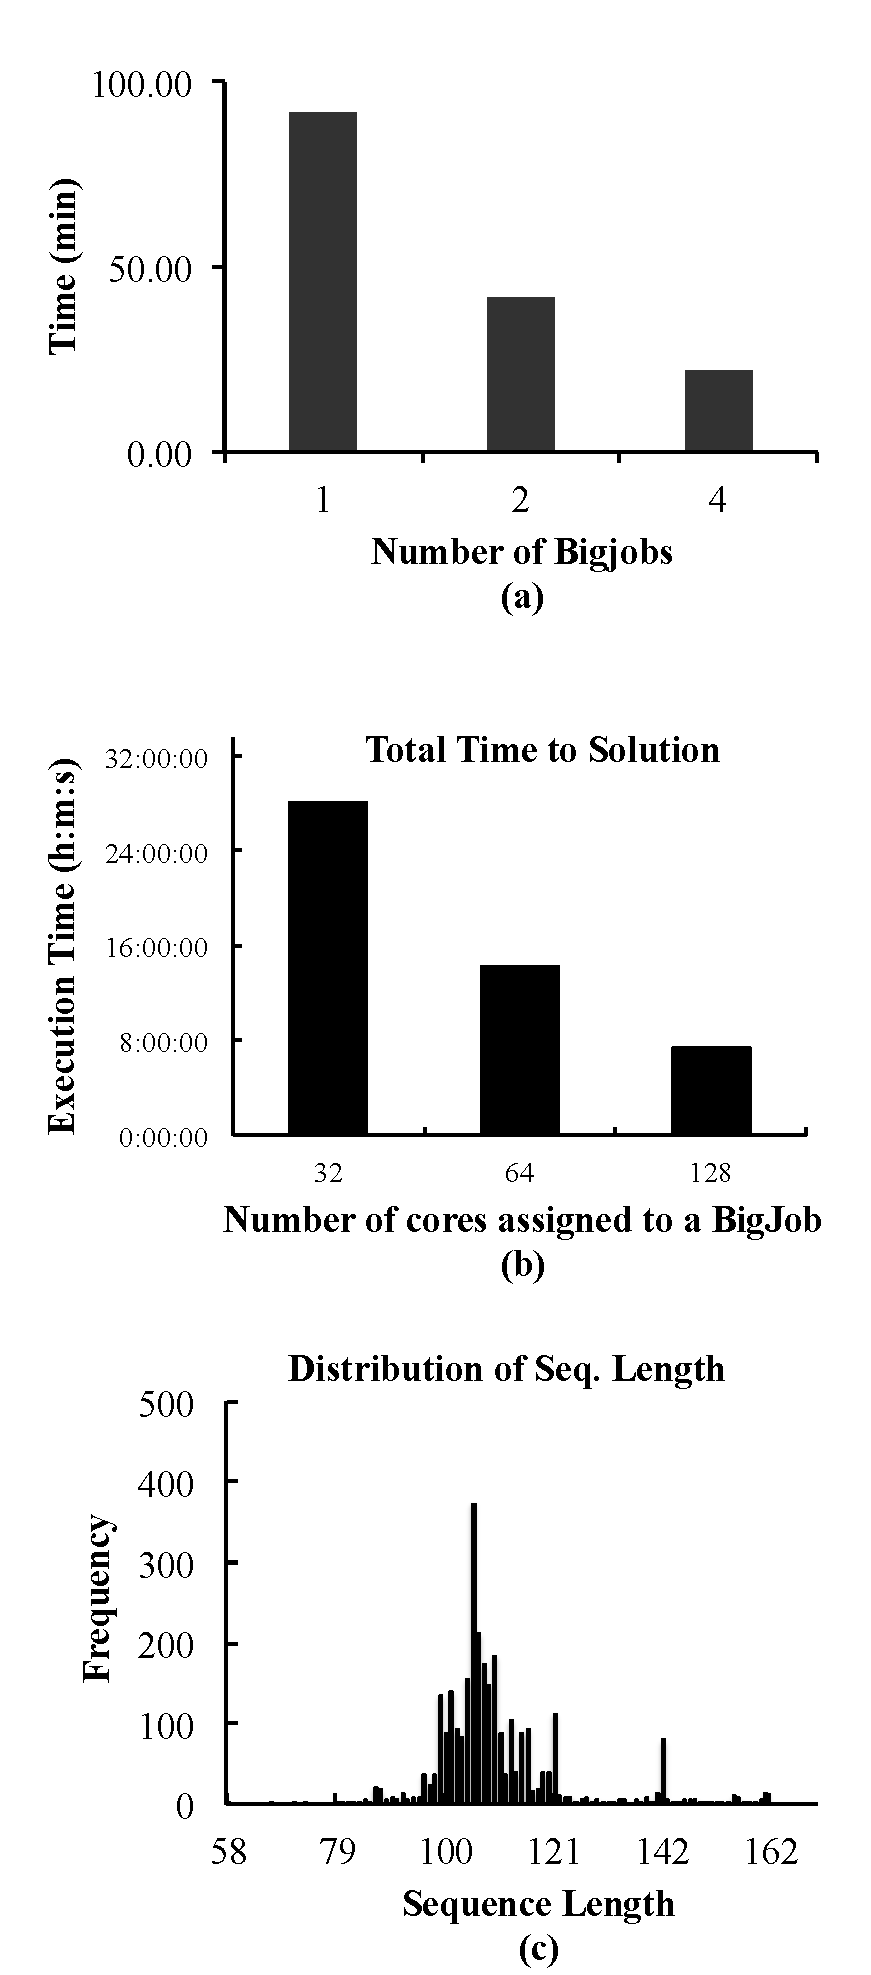
\includegraphics[scale=0.50]{figures/dare-rfold-result.pdf}

\caption{\small Massive concurrent calculation capability is presented with the results obtained with DARE-Rfold. The total 2910 SAM-I riboswitch sequences are injected into the DARE-Rfold for sampling of Boltzman-weighted secondary structures.  SAGA-BigJob handles these many tasks by decoupling the resource assignment and execution of each task, collectively allowing an efficient management of many tasks. In (a) and (b), time-to-solutions with different configurations of BigJob are compared in terms of the number of BigJobs (a) and the size of a BigJob (b).  In (c), the distribution of sizes of 2910 input sequences is illustrated.  This distribution is directly associated with the distribution of time-to-solutions of all 2910 tasks.}
  \label{fig:dare-rfold-result} 
\end{figure}



\subsection{DARE-Dock}
DARE-Dock was developed to support the basic virtual screening and the target application is Autodock\cite{autodock}.  Autodock-vina is provided as a main tool to utilize its support for fine-grain parallelism with multi-threading multi-core support, whose capability is thus considerably enhanced with task level concurrency implemented with pre-processing that breaks the set of ligands in a given chemical database into many sets\cite{autodock-vina}.  


\subsection{DARE-HTHP}




\subsection{Achieving IDEAS : Interoperability, Distributed scaled-out, Extensibility, Adaptivity, and Simplicity}
\smnote{ 1) Lets say we have "n" read files and with DARE it takes around time "t" time for matching step if we run it serially it would take n*t time. It probably exceeds wall time limit. Therefore speed up in match step depends how many number of read files we generate and process concurrently.
2) Yes we were able to process the complete run with entire Human Genome on QB and Ranger separately. (**I am currently working this to utilizing QB and Ranger together.) 
4) it should clearly provide the advantage with multiple resources. If we want to use the cloud resources from India to complete Human Genome run it is not practically possible because of the current limited disk size access provided by the FG Eucalyptus resources. Because whole human genome index files are of size 129 GB for Bfast matching step as opposed to HG 18 Chromosome 21 with size of  2 GB index files. On the other hand it also requires the temporary files disk space.  Thus it is important to utilize large capacity resources like QB and Ranger divide the work load across machines.}
Here, we present how the objectives of IDEAS are accomplished with the DARE gateway examples.  First of all, the theme of Simplicity is considered from the underlying SAGA-based API, through a Pilot-Job abstraction, SAGA-BigJob, and the design of the DARE architecture.  All of components in the DARE framework are independent to each other due to its modular structure.  Additionally, the framework provides the key functionality for job management and data management with heterogeneous distributed resources in a flexible mechanism to support various execution patterns and application usage modes as well as the full-fledge access layer with the web server framework.  Along with this backbone template, a developer can quickly implement his/her own scientific logics in the application layer with python scripts.  Secondly, the theme of Distributed scaled-out might be illustrated with Table~\ref{table:NGS-Distributed}.  Here, two large TeraGrid systems, QB and Ranger, were used for the match step in BFAST pipeline.  It is noticeable that we compare different usage modes, for example, using one resource or two resource altogether with the same configuration for the computation.  As we demonstrated in numerous publications, having more resources and using those scaled computing power benefits to decrease the time-to-completion.  The results of the cases in Table~\ref{table:NGS-Distributed} indicate also there are interesting aspects due to the complexity of scientific applications.  For example, in the NGS data alignment using BFAST, we should consider the optimal condition with the task level concurrency considering how the reference genome indexes are utilized for chucks of short read data\cite{ecmls11}.  Extensibility is an important theme in our DARE-based gateway development, and indeed, many levels of extensibility are easily utilized.  While SAGA itself provide the capabilities to expand its lineup with various adaptors to deal with emerging new environment such as clouds, SAGA and SAGA-BigJob, combined together, provides great flexibility to extend scientific capability of a gateway. For example, with DARE-Rfold, we attempted to make a pipeline for another capability beyond RNA secondary structure prediction.  We demonstrated recently the output from the RNA secondary structure prediction could be utilized for Riboswitch gene annotation with structural information.  Furthermore, with the open source pylons framework, incorporation of many web technologies is achieved efficiently.  Interoperability is what SAGA-based approaches enjoys in a full scale with numerous adaptors as well as support of programming models such as MapReduce.  Finally, Adaptivity is importantly dealt with in the design of the DARE framework.  SAGA-BigJob has many advantages to be agile to change the application usage mode from one to the other.  In Fig.~\ref{fig:dare-rfold-result}, the result compares with two different configurations of BigJob size, for example.  Note that not only varying the size of a BigJob, other possible usage modes supporting a case of loosely coupled applications and a case of dynamically changing parallel/concurrent configurations in the fine-grain parallelization (for example, MPI configuration) as well as the coarse-grain parallelization are effectively designed. 








\bibliographystyle{abbrv}
\bibliography{tg11}




\end{document}

